\chapter{Preface}

This document is for newcomers to MOLE (Mimetic Operator's
Library Enhanced) with a solid foundation in numerical analysis for
Partial Differential Equations (PDEs).
The library's algorithms are continuously evolving, with examples
implemented in
\href{https://octave.org}{GNU Octave}/\href{https://www.mathworks.com/products/matlab.html}{MATLAB}
and \href{https://isocpp.org}{C++} using the Armadillo sparse linear
algebra library.
Currently, these are only two language implementations available.
However, mastering this content will enable users to translate the
algorithms into other high-performance
scientific programming languages, such as
\href{https://julialang.org}{Julia},
\href{https://www.python.org}{Python},
\href{https://fortran-lang.org}{Fortran},
\href{https://www.open-std.org/jtc1/sc22/wg14}{C} and
\href{https://www.rust-lang.org}{Rust}.

The main goal of this manual is to provide clear explanations and
complete examples to help users understand the core
concepts and applications of the library.

We would like to thank Professor
\href{https://ctivitae.concytec.gob.pe/appDirectorioCTI/VerDatosInvestigador.do?id_investigador=45848}{Miguel Dumett}
of the Computational Science Research Center at San Diego State
University and the National University of Trujillo for organizing
MOLE courses.

\begin{figure}[ht!]
	\centering
	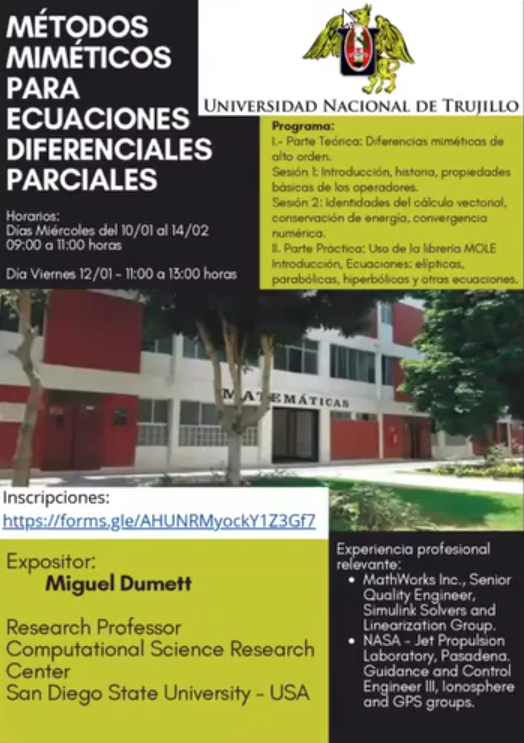
\includegraphics[width=.32\paperwidth]{mole2024}\quad
	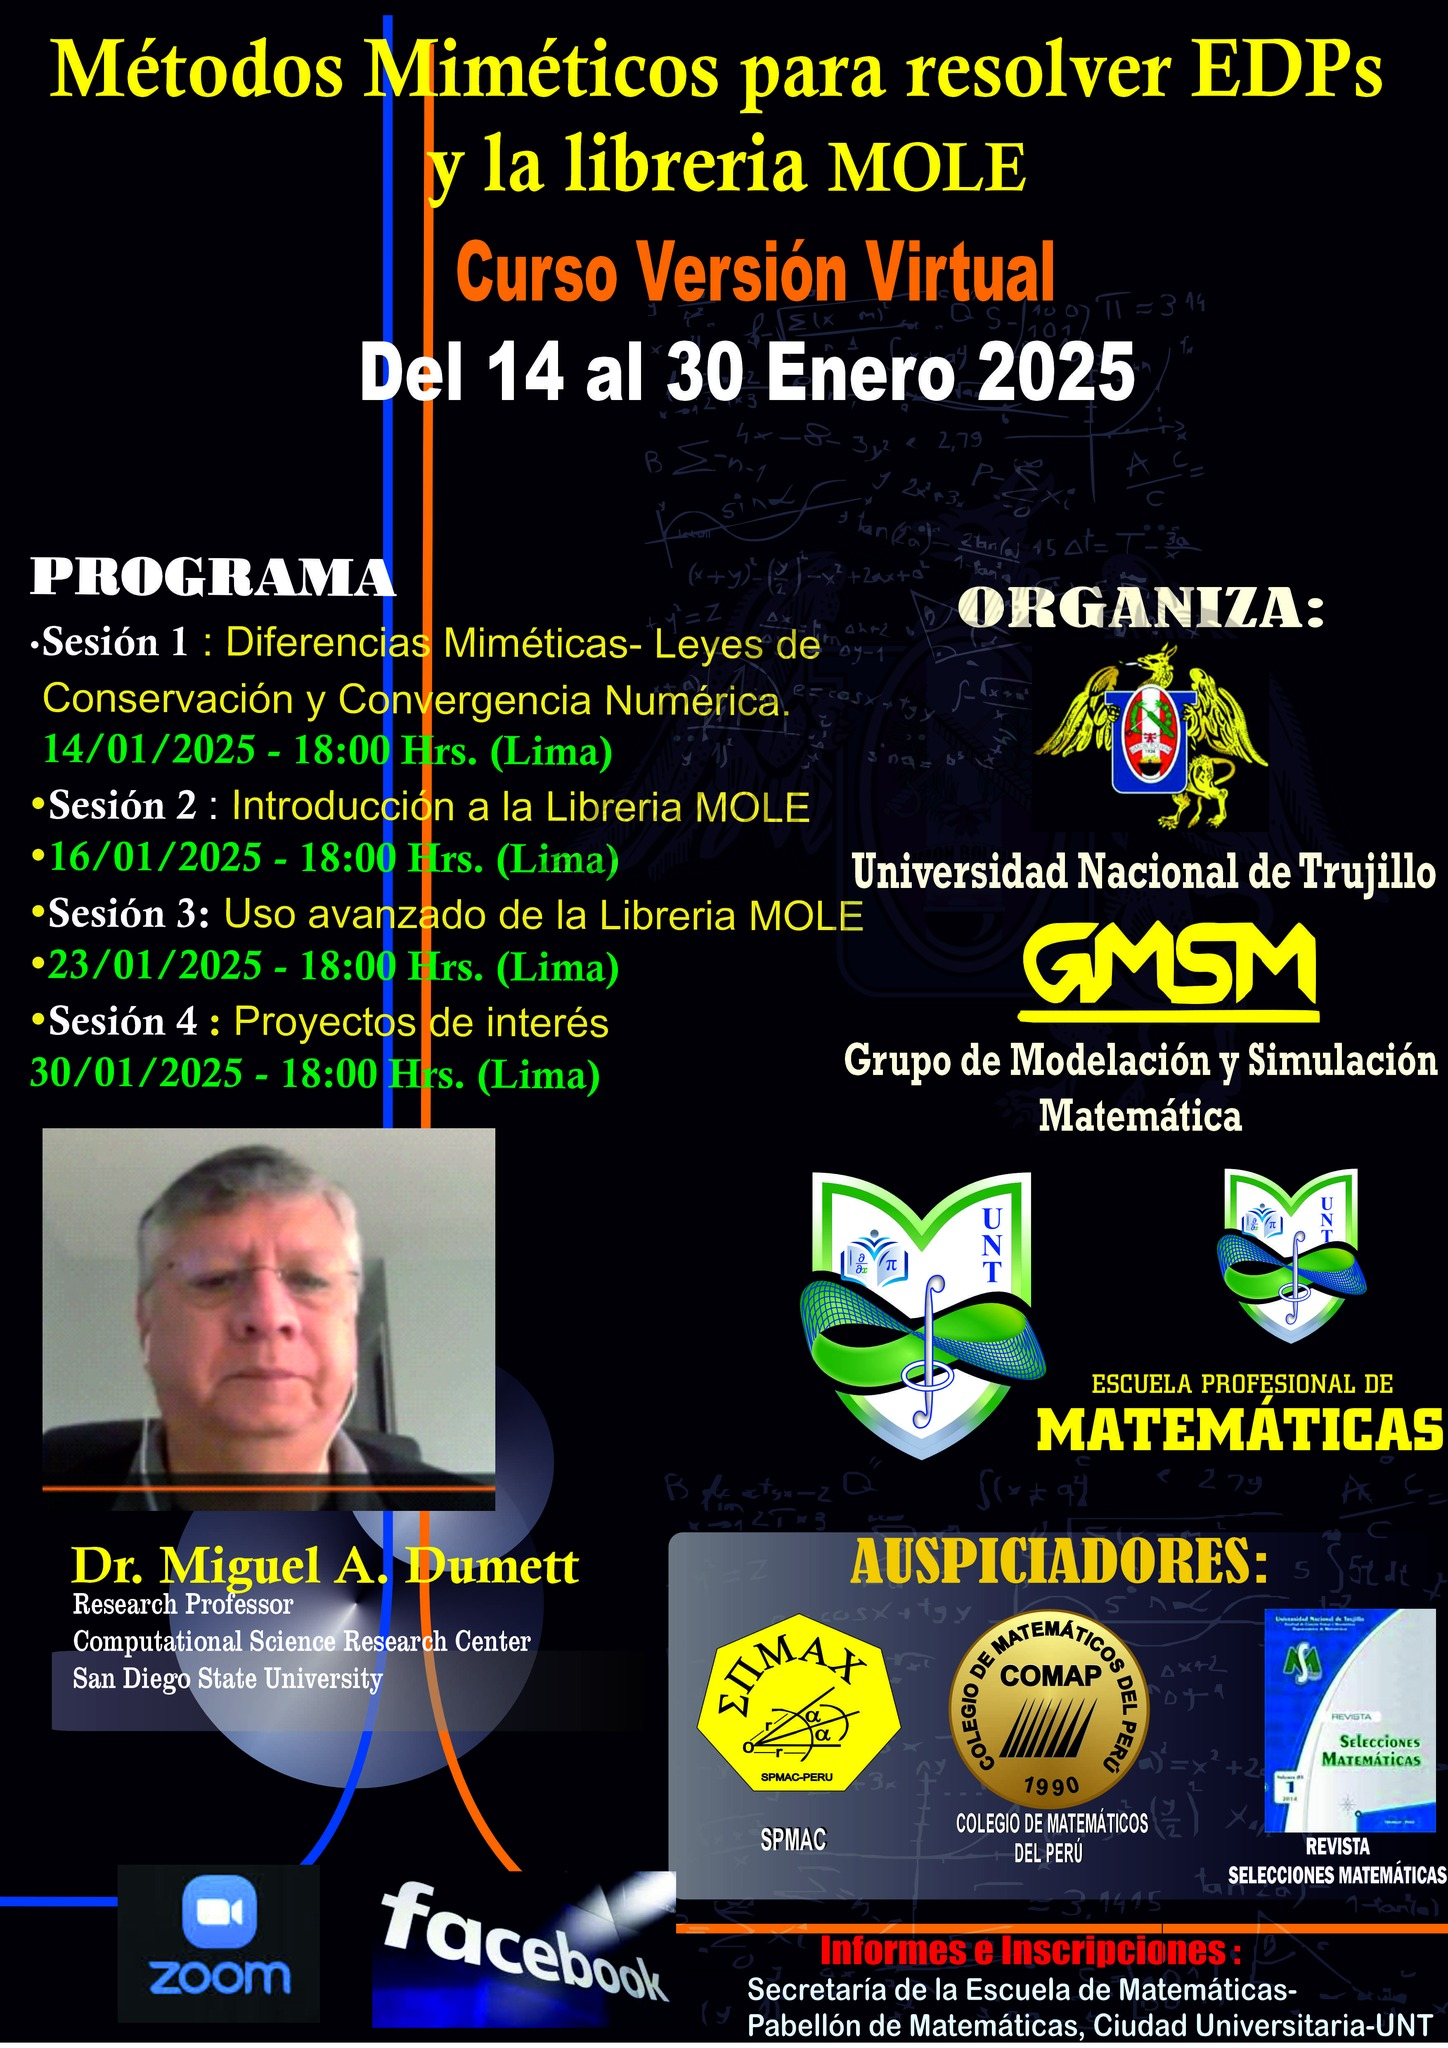
\includegraphics[width=.32\paperwidth]{mole2025}
	\caption*{\bfseries Mimetic Methods courses in January and February 2024 and 2025.}
\end{figure}

\begin{flushright}
	Lima, Puno \hfill Carlos Aznarán \\[.5\baselineskip]

	March 2025 \hfill Adelaida Otazu
\end{flushright}
